\documentclass[titlepage]{article}
\title{Tor - The Onion Router \\ \large Ein Projekt in Network Security bei Dr Andreas Reinhardt}
\usepackage[ngerman]{babel}
\usepackage{subfigure}
\usepackage{graphicx}
\usepackage{url}
\author{Christian, Rebischke}
\begin{document}
\maketitle
\tableofcontents
\newpage

\section{Einleitung}
In den letzten Jahrzehnten ist die Menge der Daten die via das World Wide Web versendet werden rasant angestiegen. Ebenso angestiegen ist jedoch die Anzahl der Staaten die versuchen sich das World Wide Web als Machtinstrument zu sichern. Gerade die letzten Jahre im Zusammenhang mit der Snowden-Aff"are haben uns gezeigt in welchem Umfang einige Staaten "Uberwachung und Spionage betreiben. Aber auch der Arabische Fr"uhling hat uns klar gemacht, welche Macht das Volk haben kann wenn es Zugang zum Netz hat. Da ist es nicht verwunderlich, dass einige Staaten das Netz filtern oder zensieren wollen um ihren Status Quo zu st"arken und beizubehalten. Genau an dieser Stelle kommt \textbf{Tor} ins Spiel. \textbf{Tor} ist das Akronym f"ur \textbf{The Onion Router}. Mit der Hilfe von \textbf{Tor} ist es m"oglich der Zensur eines Staates oder der permanenten "Uberwachung des Netz zu entgehen.

\section{Modus Operandi der Netz"uberwachung und Netzzensur}
Bevor wir uns n"aher mit \textbf{Tor} befassen ist es sinnvoll sich erstmal vor Augen zuf"uhren welche Arten der Netz"uberwachung und Netzzensur existieren. Am verbreitesten ist eine Zensur auf Basis des Providers wie sie beispielsweise gerade in "Osterreich im Tatbestand der Urheberrechtsverletzung stattfindet. \cite{kinox} Dort werden einfach via \textit{DNS-Filter} die DNS-Anfragen f"ur diverse Internetseiten umgeleitet. In anderen Gegenden der Welt kommen jedoch auch \textit{Content-Filter} zum Einsatz. \textit{Content-Filter} kann man noch unterteilen in diverse ``H"artegrade''. Gemeinsam haben aber alle, dass nach Content also nach Inhalt gefiltert wird. Dies kann man erreichen durch \textit{Deep Packet Inspection}, einer Technik bei der beispielweise bei TCP-Paketen die Nuztlast "uberpr"uft wird und je nach Auffinden von bestimmten Begriffen dann das Paket nicht am Ziel ankommt. Ansonsten gibt es noch Software-seitige Content-Filter die besonders gerne in Internet Cafes eingesetzt werden (so passiert in Myanmar \cite{myanmar}). Ebenfalls denkbar ist aber auch das gezielte Sperren von IP-Adressen, Filterung anhand der URL und ein sogennanter \textit{Connection Reset} der weitere Verbindungsversuche unter Verwendung des \textit{TCP-RESET-Pakets} verhindert. Das wohl bekannteste Beispiel von Internetzensur ist China mit dem \textit{Projekt Goldener Schild} hierzulande auch \textit{Gro"ße Firewall von China} genannt. Das \textit{Projekt Goldener Schild} verbindet viele der oben genannten Vorgehensweisen.

\newpage
\section{Wieso Tor?}
Eine der Kernfragen die man sich "uber \textbf{Tor} stellt ist ``Was macht \textbf{Tor} eigentlich besser als die Alternativen?''. Schauen wir uns dazu mal einige dieser Alternativen an:

\begin{itemize}
\item Lokale Webhoster
\newline
Lokale Anbieter von Internetseiten k"onnten die von der lokalen Regierung gesperrten Inhalte im Ausland lokal anbieten. So m"usste zum Beispiel im Falle von China der Traffic nicht erst die Great Firewall of China passieren. Der Nachteil ist allerdings, dass der Webhoster eine Lizenz ben"otigt und vermutlich Rechtliche Schwierigkeiten bekommt wenn so ein \textit{Spiegeln} der Internetseite publik wird.
\item Socks- oder HTTP-Proxy
\newline
Beim Socks- oder HTTP-Proxy wird einfach ein anderer Rechner zwischen die Verbindung geschaltet. Diese Art von Proxy wird meistens zum Anonymisieren einer Verbindung benutzt.
Schwachpunkt an dem System ist, dass es nicht für jedes Protokoll und jede Anwendung Proxys gibt. Außerdem findet nicht bei jeder Verbindung eine Verschl"usselung statt, sondern nur wenn beispielsweise auch HTTPS verwendet wird. Dadurch das es sich meistens nur um ein System handelt ist es f"ur den "uberwachenden Staat auch sehr einfach zur"uckzuverfolgen wer auf welchen Proxy zugegriffen hat. Liegt der Proxy im eigenen Land w"are es sogar denkbar "uber den f"alschlicherweise als Proxy herausgegebenen Server den gesamten Internetverkehr zu sniffen der "uber diesen Proxy l"auft. Der Proxy l"auft also  Anwendungsspezifisch auf \textit{OSI-Layer 7}.
\item VPN (Virtual Private Network)
\newline
Der VPN ist vergleichbar mit einem Proxy. Ein VPN arbeitet jedoch auf \textit{OSI-Layer 3} oder sogar \textit{OSI-Layer 2}. Dies macht den VPN unabh"angig von der Anwendung. Der gesamte Rechner h"angt sozusagen in einem anderen Netz, der gesamte ausgehende Traffic vom Client geht nach Verbinden mit dem VPN-Server "uber diesen VPN-Server. Hizukommt, dass viele VPNs eine starke Verschl"usselung anbieten oder sogar das IPSec-Protokoll unterst"utzen wie beispielsweise \textit{Strongswan}. Nachteile des VPNs sind "ahnlich wie beim Proxy. Die jeweilige Regierung kann die IPs von dem VPN-Anbieter blacklisten, den VPN-Anbieter juristisch in die Mangel nehmen (falls er in juristischer Reichweite liegt) oder einfach ohne dem Wissen des VPN-Anbieters dessen Knoten "uberwachen und schauen was rein geht und was rauskommt.
\end{itemize}
Zusammengefasst kann man die Schwachpunkte der oben genannten Methoden als zu stark ausgepr"agt betrachten als, dass sie wirklich eine sinnvolle Ma"snahme gegen Netzzensur wie beispielsweise in China darstellen. Keine der oben genannten Methoden bietet eine Sicherheit auf Anonymit"at die Oppositionelle oder Whistleblower dringend n"otig haben.
\newline
Dies ist der Grund f"ur \textbf{Tor}.

\newpage
\section{Grundlegende Prinzipien von Tor}
Die grundlegenden Prinzipien von \textbf{Tor} sind denkbar einfach. Wie man aus dem Namen bereits schlie"sen kann ist \textbf{Tor} aufgebaut wie eine Zwiebel. Au"serdem besitzt \textbf{Tor} das Prinzip des \textit{Darknet}. Mehrere \textbf{Tor}-Knoten bilden also praktisch ein eigenes Intranet auf das wiederum nur \textbf{Tor}-Clients oder andere \textbf{Tor}-Knoten zugreifen k"onnen. Jeder \textbf{Tor}-Knoten kann eine einkommende Verbindung an einen weiteren \textbf{Tor}-Knoten weiterreichen. Sogenannte \textit{Tor-Exit-Nodes} k"onnen dann eine Verbindung ins ``echte Internet'' herstellen. Es lassen sich beliebig viele dieser \textbf{Tor}-Knoten kaskadieren. Dadurch wird es "au"serst schwierig f"ur "Uberwachungsorgane festzustellen welche Verbindung zu welchem \textbf{Tor}-Nutzer geh"ort. Durch den Zwiebel-Artigen Aufbau ist die gesamte Verbindung verschl"usselt und jeder \textbf{Tor}-Knoten kennt nur seinen Nachfolger.
\begin{figure}[h]
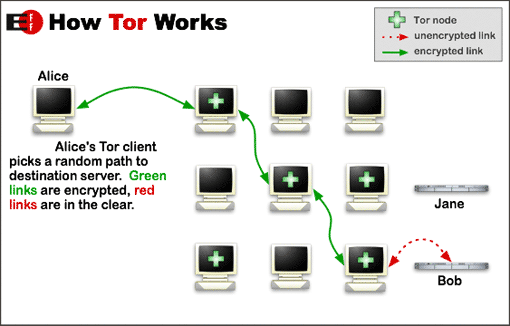
\includegraphics[scale=1.0]{tor}
\centering
 \caption{The Onion Router Netzwerk}
 \label{tor}
\end{figure}

\newpage
\section{Technische Details}
\subsection{Bestandteile des Tor-Netzwerks}
Das \textbf{Tor}-Netzwerk hat folgende Bestandteile:
\begin{itemize}
\item Entry Guards
\newline
Entry Guards sind sowas wie die W"achter des \textbf{Tor}-Netzwerks. Die Idee f"ur Entry Guards kam auf als klar wurde, dass ein Angreifer einen oder mehrere \textbf{Tor}-Nutzer deanonymisieren kann wenn er Kontrolle "uber den Start und Endknoten hat. Alleine "uber die genaue Paketanzahl und zeitliche Abfolge k"onnte man einen Nutzer auf Dauer deanonymisieren.
Um dies zu verhindern hat man feste Startknoten eingef"uhrt. sogenannte Entry Guards. Somit sind die Startknoten statisch, nicht dynamisch wie man erst erwarten w"urde. Dadurch kann man die gesamte Anzahl der \textbf{Tor}-Nutzer auf einige Entry Guards verteilen. Dies hat zur Folge, dass der Angreifer (falls er einen Startknoten kontrolliert) immer nur die selbe Anzahl an Verbindungen bekommt. Somit l"asst sich nicht mehr die aktuelle Zahl an \textbf{Tor}-Nutzern durch den Angreifer ermitteln. A"u"serdem verhindert dies eine "Uberwachung der Nutzer wenn beispielsweise eine Route gew"ahlt wird mit Entry-Guards die nicht vom Angreifer kontrolliert werden. Wenn ein Nutzer jedoch einen komprommierten Entry-Guard erwischt erh"oht dies die Chance auf Deanonymisierung wenn der Angreifer zuf"alligerweise noch beispielsweise den Exit-Node komprommitiert hat.
\item Exitnodes
\newline
Exitnodes sind sowas wie die Fenster vom Onion-Netz in das richtige Internet. Sie bilden einen Ausgang aus dem \textbf{Tor}-Netzwerk. Dadurch das der Exitnode nur den letzten Knoten in der Kaskade kennt ist es "au"serst schwierig den genauen Urheber der Verbindung zu 
ermitteln.
\item Hiddenserver
\newline
Die sogenannten Hiddenserver sind Server im \textbf{Tor}-Netzwerk. Jeder \textbf{Tor}-Knoten kann auch zu gleich als Hiddenserver fungieren. Durch Hiddenserver ist es m"oglich nicht mehr das komplettverschl"usselte \textbf{Tor}-Netzwerk zu verlassen um auf Inhalte zuzugreifen. So l"asst sich praktisch fast jeder Dienst als Hiddenserver betreiben. Angefangen bei einfachen Webservern bis hinzu SSH-Server. Beim Erstellen des Hiddenservers wird eine im \textbf{Tor}-Netzwerk eindeutige URL erstellt mit der Endung \textit{.onion}. Anhand dieser URL kann man dann den Server ansprechen. Der Einsatz von Hiddenserver macht das Netzwerk um ein Vielfaches sicherer, da Traffic nun nicht mehr unbedingt "uber abh"orbare Exitnodes laufen muss sondern im verschl"usselten \textbf{Tor}-Netzwerk bleibt. Desweiteren kann so ein Aufenthaltsort und Eigent"umer des Hiddenservers komplett verschleiert werden. Client-Nutzer und Server-Inhaber bleiben so komplett anonym und k"onnen Inhalte tauschen. Diese Technik nennt man auch `` Rendezvous-Punkt''.
\item Directoryserver
\newline
Directoryserver bieten eine Art Inhaltsverzeichnis "uber die \textbf{Tor}-Knoten an. Bei jedem Verbindungsaufbau zum \textbf{Tor}-Netzwerk wird eine komplette Liste aller verf"ugbaren Knoten heruntergeladen.
\item Bridges
\newline
Die Bridges sind der ma"sgebende Ausschlagpunkt wieso \textbf{Tor} in so vielen Zensurbehafteten Staaten erfolgreich eingesetzt wird. Da alle Knoten durch die Directoryserver "offentlich bekannt sind ist es f"ur Staaten besonders einfach diese komplette Liste zu sperren. Um den B"urgern trotzdem einen Zugriff auf das Netzwerk zu erm"oglichen kann jeder Client auch als Bridge konfiguriert werden. Die genauen Kontaktdaten f"ur diese Bridge k"onnen dann m"undlich oder elektronisch weitergegeben werden oder bei einer \textit{Bridge Authority} hinterlegt werden. \cite{blocking}
\item Bridge Authority
\newline
Die Bridge Authority besteht aus 3 Pools. Pool 1 verteilt die Bridge-Adressen via Web. Pool 2 verteilt die Bridge-Adressen via Email und Pool 3 via Soziale Netzwerke. Dies macht es "au"serst schwierig den Zugang zum \textbf{Tor}-Netzwerk zu unterbinden.
\end{itemize}

\newpage
\subsection{Verbindungsablauf}
Abbildung 2 soll den Aufruf von http://www.google.de via \textbf{Tor} erl"autern:
\newline
\begin{figure}[h]
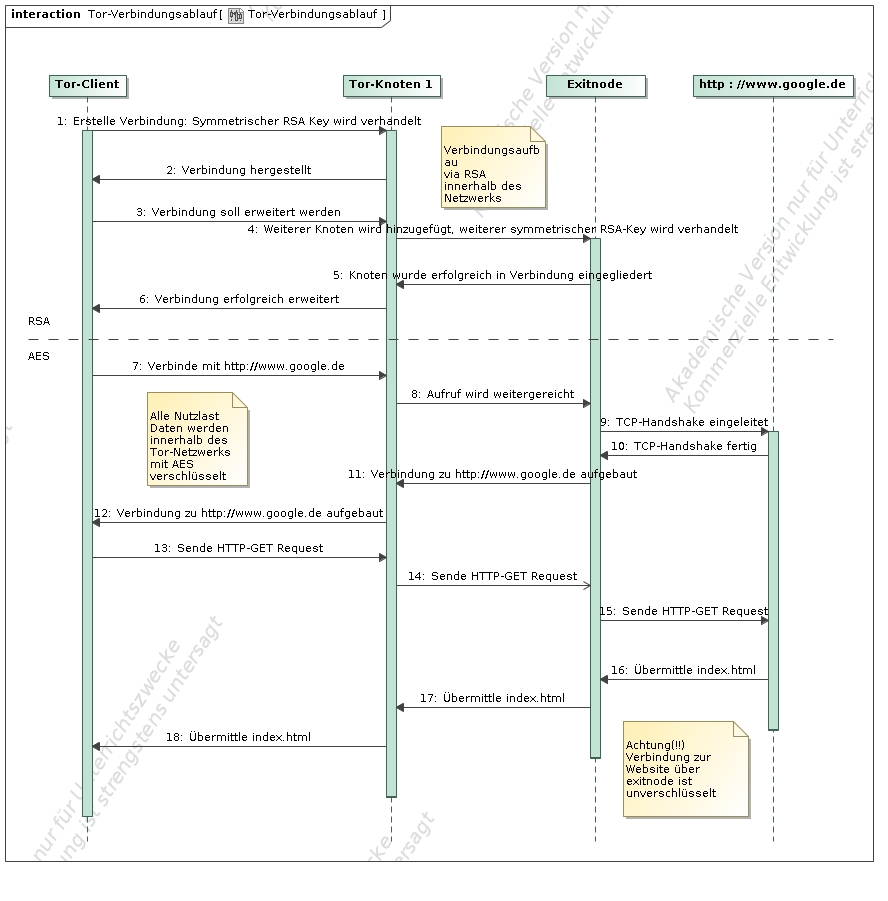
\includegraphics[scale=0.4]{Verbindungsablauf}
\centering
 \caption{Tor-Verbindungsaufbau}
 \label{Verbindungsablauf}
\end{figure}

Erl"auterung: Beim Verbindungsaufbau vom Client zum ersten Knoten wird ein symmetrischer RSA Schl"ussel benutzt. Dieser Schl"usselbund wird dann f"ur jede weitere Erweiterung der Verbindung inkrementiert. Pro Knoten ein symmetrischer RSA-Schl"ussel mehr. Der symmetrische RSA-Key ist daf"ur da um die Nutzlast zu verschl"usseln: Einen Diffi-Hellman-Handshake. Ist die Verbindung hergestellt werden alle Nutzerdaten innerhalb des \textbf{Tor}-Netzwerks mit AES verschl"usselt. \cite{design} Das Obige Beispiel verdeutlicht gut wieso Hiddenserver so wichtig sind. Denn die Verbindung zwischen Exitnode und Website ist nicht mehr AES verschl"usselt. In unserem Beispiel sogar nichtmal SSL verschl"usselt weil nicht die HTTPS-Instanz von Google aufgerufen wird.

\newpage
\section{Fazit}
Es ist nun eindeutig klar, dass \textbf{Tor} eine sichere Alternative zu VPN und Proxies ist.
Durch die Kaskadierung der einzelnen Tor-Knoten wird eine h"ohere Anonymit"at als bei VPN oder Proxy gew"ahrleistet. Ausserdem bietet \textbf{Tor} einen besseren Weg Zensurma"snahmen wie die von China zu umgehen. Auch wenn es China immer wieder (unter Einsatz von Deep Packet Inspection) gelingt den Zugriff auf alle Bridges zu unterbrechen, in dem sie systematisch nach spezifischen \textbf{Tor}-Traffic suchen und die entsprechenden Verbindungen nullrouten. 
\newpage
\section{Quellen}
\nocite{*}
\bibliography{quotes}
\bibliographystyle{plain}
\listoffigures
\end{document}
